\documentclass[]{article}
\usepackage{graphicx}
\usepackage{subcaption}
\usepackage{tikz}
\usetikzlibrary{fit}
\usetikzlibrary {arrows.meta,graphs,shapes.misc}
\usetikzlibrary {positioning}
\pagenumbering{gobble}
\usepackage{tikz-network}
\begin{document}

% point triangle
\begin{figure}
	\centering
	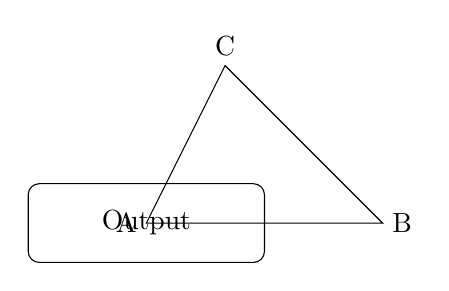
\begin{tikzpicture}
		\tikzstyle{rect} = [rectangle, rounded corners, minimum width=3cm, minimum height=1cm,text centered, draw=black]
		\tikzstyle{arrow} = [thick,->,>=stealth]
		\node (output) [rect] {Output};
		\draw   (0,0) coordinate[label= left:A] (a) -- 
		(3,0) coordinate[label=right:B] (b) -- 
		(1,2) coordinate[label=above:C] (c) -- cycle;
	\end{tikzpicture}
\end{figure}


\end{document}
